\subsection{Constructing SCC Tree}

We will look at the construction of the SCC tree for the graph shown in \figureref{\ref{fig:graph1}}.
We start by finding all the SCCs of the graph and then construct the SCC-Tree for each SCC in it.
In the process of finding all the SCCs, we would also fill the SCC mapping array. 
A special tree node \textsc{STN}(M), called the master node would preserve the connectivity of the SCCs (condesed form of the original graph).
Suppose we have a strongly connected graph $G$, the SCC Tree for the graph is constructed as follows:
\begin{itemize}
    \item If $|V(G)| = 1$ and $v \in V(G)$, then the SCC tree is $SCC(v) = STN(v) = (\{v\}, \emptyset)$.
    \item If $|V(G)| > 1$ and $d \in V(G)$, then SCC-tree node would contain the graph \textsc{Condense}(\textsc{Split}($G, d$)), 
    and for each SCC in the graph \textsc{Condense}(\textsc{Split}($G, d$)), we add its SCC-tree as a subtree of R, with 
    exception that we would add only one tree for vertex $d$ instead of $d_{in}$ and $d_{out}$.
\end{itemize}

\begin{algorithm}
    \SetAlgoLined
    \KwData{G}
    \KwResult{SCC mapping, \textsc{SccTree}s, \textsc{STN}(M)}
    $SM_{G} = \emptyset, \textsc{SccTree} = \emptyset$\;
    $S = \textsc{FindSccs}(G), V_l = \emptyset, E_l = E(G)$\;
    \For {each $s \in S$} {
        $L_s = \textsc{Label}(s)$\;
        $G_s = G \cap s$\;
        $\textsc{SccTree}(L_s) = \textsc{MakeTree}(G_s, L_s)$\;
        \For {each $v \in s$} {
            $SM_{G}(v) = L_s$\;
        }
        $V_l = V \cup \{L_s\}$\;
        $E_l = E_l - \{e \in E(G_s)\}$\;
    }
    $\textsc{STN}(M) = (V_l, E_l)$\;
    \Return $SM_{G}, \textsc{SccTree}s, \textsc{STN}(M) = (V_l, E_l)$\;

    \caption{\textsc{ConstructDS}(G)}
\end{algorithm}

\begin{figure}[H]
    \centering
    \begin{subfigure}{0.45\textwidth}
        \centering
        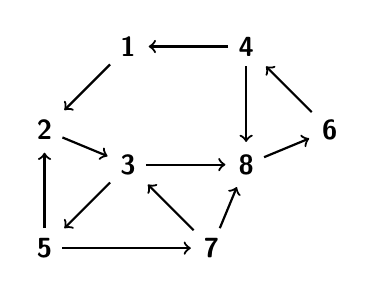
\begin{tikzpicture}[->,shorten >=1pt,auto,node distance=1.5cm,
            thick,main node/.style={font=\sffamily\bfseries}]

        % Define vertices
        \node[main node] (1) {1};
        \node[main node] (2) [below left of=1] {2};
        \node[main node] (3) [below of=1] {3};
        \node[main node] (4) [right of=1] {4};
        \node[main node] (5) [below left of=3] {5};
        \node[main node] (6) [below right of=4] {6};
        \node[main node] (7) [below right of=3] {7};
        \node[main node] (8) [right of=3] {8};
        

        % Draw edges
        \path[every node/.style={font=\sffamily\small}]
            (1) edge (2)
            (2) edge (3)
            (3) edge (5)
            (3) edge (8)
            (4) edge (1)
            (4) edge (8)
            (5) edge (2)
            (5) edge (7)
            (6) edge (4)
            (7) edge (3)
            (7) edge (8)
            (8) edge (6);

        \end{tikzpicture}
        \caption{Graph 1}
        \label{fig:graph1}
    \end{subfigure}
    \hfill
    \begin{subfigure}{0.45\textwidth}
        \centering
        
\begin{tikzpicture}[->,shorten >=1pt,auto,node distance=2cm,
            thick,main node/.style={circle,draw,font=\sffamily\bfseries}]

        % Define vertices
        \node[main node] (R) {R};

        \end{tikzpicture}
        \caption{condensed graph 1}
        \label{fig:condensed_graph1}
    \end{subfigure}
    \caption{Graph 1 and its condensed graph}
    \label{fig:graph1_and_condensed_graph1}
\end{figure}


%algorithm
\begin{algorithm}
    \SetAlgoLined
    \KwData{G | G is strongly connected, L | label of the root node}
    \KwResult{\textsc{SccTree(L)}}
    $v = random(V(G))$\;
    $\textsc{SccTree}(L) = \emptyset$\;
    \If {$|V(G)| = 1$} {
        $\textsc{STN}(L) = (\{v\}, \emptyset)$\;
        $\textsc{SccTree}(L) = \textsc{STN}(L)$\;
        \Return \textsc{SccTree}(L)\;
    }
    $G' = \textsc{Split}(G, v)$\;
    $S = \textsc{FindSccs}(G')$\;
    \For {each $s \in S$ and $v_{in} \not \in s$} {
        $L_s = \textsc{Label}(s)$\;
        $G_s = G' \cap s$\;
        $\textsc{SccTree}(L_s) = \textsc{MakeTree}(G_s, L_s)$\;
        $\textsc{SccTree}(L) = \textsc{SccTree}(L) \cup \textsc{SccTree}(L_s)$\;
    }
    $\textsc{STN}(L) = \textsc{Condense}(G')$\;
    $\textsc{SccTree}(L) = \textsc{SccTree}(L) \cup \textsc{STN}(L)$\;
    \Return \textsc{SccTree}(L)\;

    \caption{\textsc{MakeTree(G, L)}}
\end{algorithm}

We can understand the algorithm by looking at the following figures.
In \figureref{\ref{fig:graph1_and_condensed_graph1}}, we have the graph $G$, which is strongly connected.
Its condensed form would contain a single node $R$. The SCC mapping array would map all the nodes to $R$ and the master node 
would contain the graph in \figureref{\ref{fig:condensed_graph1}}.

After the strongly connected components of the graph are indentified, they are individually processed by the 
\textsc{MakeTree} algorithm. The algorithm starts by selecting a random vertex from the SCC and then splits the graph
on that vertex. The split graph is then condensed and the strongly connected components of the condensed graph are found. 
This is illustrated in \figureref{\ref{fig:scc_r_split_and_condensed_graph1}}, where we can see the condensed components $A$ and $B$.
The condesed graph in \figureref{\ref{fig:condensed_scc_r_split}} is stored in the \textsc{STN} of the root node $R$.
\begin{figure}[H]
    \centering
    \begin{subfigure}{0.45\textwidth}
        \centering
        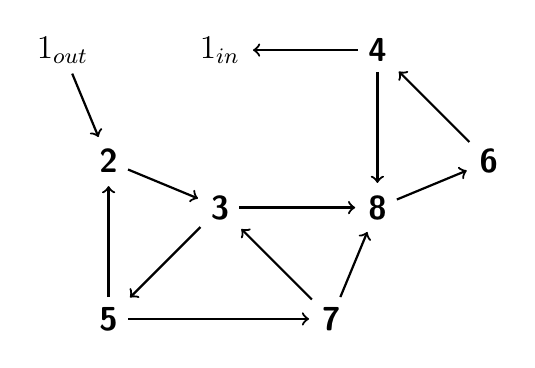
\begin{tikzpicture}[->,shorten >=1pt,auto,node distance=2cm,
            thick,main node/.style={font=\sffamily\large\bfseries}]

        % Define vertices
        \node[main node] (1) {$1_{in}$};
        \node[main node] (11) [left of=1] {$1_{out}$};
        \node[main node] (2) [below left of=1] {2};
        \node[main node] (3) [below of=1] {3};
        \node[main node] (4) [right of=1] {4};
        \node[main node] (5) [below left of=3] {5};
        \node[main node] (6) [below right of=4] {6};
        \node[main node] (7) [below right of=3] {7};
        \node[main node] (8) [right of=3] {8};
        

        % Draw edges
        \path[every node/.style={font=\sffamily\small}]
            (11) edge (2)
            (2) edge (3)
            (3) edge (5)
            (3) edge (8)
            (4) edge (1)
            (4) edge (8)
            (5) edge (2)
            (5) edge (7)
            (6) edge (4)
            (7) edge (3)
            (7) edge (8)
            (8) edge (6);

        \end{tikzpicture}
        \caption{SCC(R) split on 1}
        \label{fig:scc_r_split}
    \end{subfigure}
    \hfill
    \begin{subfigure}{0.45\textwidth}
        \centering
        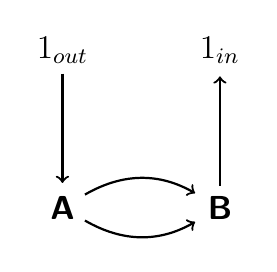
\begin{tikzpicture}[->,shorten >=1pt,auto,node distance=2cm,
            thick,main node/.style={font=\sffamily\large\bfseries}]

        % Define vertices
        \node[main node] (1) {$1_{in}$};
        \node[main node] (11) [left of=1] {$1_{out}$};
        \node[main node] (A) [below of=11] {A};
        \node[main node] (B) [below of=1] {B};
        

        % Draw edges
        \path[every node/.style={font=\sffamily\small}]
            (11) edge (A)
            (A) edge[bend left] (B)
            (A) edge[bend right] (B)
            (B) edge (1);

        \end{tikzpicture}
        \caption{condensed graph}
        \label{fig:condensed_scc_r_split}
    \end{subfigure}
    \caption{SCC(R) split on 1 and its condensed graph}
    \label{fig:scc_r_split_and_condensed_graph1}
\end{figure}

The \textsc{MakeTree} algorithm then processes all the condensed components of the split graph in a recursive manner.
The condensed component $A$ is split on 2, as in \figureref{\ref{fig:scc_a_split_and_condensed_graph1}}, and the 
condensed component $B$ is split on 4, as shown in \figureref{\ref{fig:scc_b_split_and_condensed_graph1}}. The 
component $A$ contains $C$ which is split on 3, as shown in \figureref{\ref{fig:scc_c_split_and_condensed_graph1}}.
The condesed graphs in \figureref{\ref{fig:condensed_scc_a_split}}, \figureref{\ref{fig:condensed_scc_b_split}}, and
\figureref{\ref{fig:condensed_scc_c_split}} are stored in the \textsc{STN} of $A$, $B$, and $C$ respectively.
\begin{figure}[H]
    \centering
    \begin{subfigure}{0.45\textwidth}
        \centering
        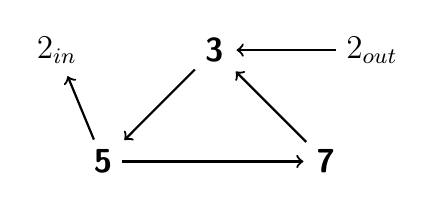
\begin{tikzpicture}[->,shorten >=1pt,auto,node distance=2cm,
            thick,main node/.style={font=\sffamily\large\bfseries}]

        % Define vertices
        \node[main node] (3) {3};
        \node[main node] (2) [right of=3] {$2_{out}$};
        \node[main node] (22) [left of=3] {$2_{in}$};
        \node[main node] (5) [below left of=3] {5};
        \node[main node] (7) [below right of=3] {7};
        

        % Draw edges
        \path[every node/.style={font=\sffamily\small}]
            (2) edge (3)
            (3) edge (5)
            (5) edge (22)
            (5) edge (7)
            (7) edge (3);

        \end{tikzpicture}
        \caption{SCC(A) split on 2}
        \label{fig:scc_a_split}
    \end{subfigure}
    \hfill
    \begin{subfigure}{0.45\textwidth}
        \centering
        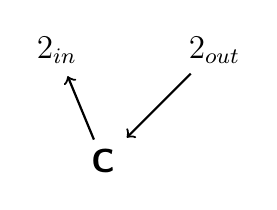
\begin{tikzpicture}[->,shorten >=1pt,auto,node distance=2cm,
            thick,main node/.style={font=\sffamily\large\bfseries}]

        % Define vertices
        \node[main node] (2) {$2_{out}$};
        \node[main node] (22) [left of=2] {$2_{in}$};
        \node[main node] (C) [below left of=2] {C};
        

        % Draw edges
        \path[every node/.style={font=\sffamily\small}]
            (2) edge (C)
            (C) edge (22);

        \end{tikzpicture}
        \caption{condensed graph}
        \label{fig:condensed_scc_a_split}
    \end{subfigure}
    \caption{SCC(A) split on 2 and its condensed graph}
    \label{fig:scc_a_split_and_condensed_graph1}
\end{figure}

\begin{figure}[H]
    \centering
    \begin{subfigure}{0.45\textwidth}
        \centering
        \begin{tikzpicture}[->,shorten >=1pt,auto,node distance=2cm,
            thick,main node/.style={font=\sffamily\large\bfseries}]

        % Define vertices
        \node[main node] (4) {$4_{in}$};
        \node[main node] (44) [left of=1] {$4_{out}$};
        \node[main node] (6) [below of=1] {6};
        \node[main node] (8) [below of=11] {8};
        

        % Draw edges
        \path[every node/.style={font=\sffamily\small}]
            (44) edge (8)
            (8) edge (6)
            (6) edge (4);

        \end{tikzpicture}
        \caption{SCC(B) split on 4}
        \label{fig:scc_b_split}
    \end{subfigure}
    \hfill
    \begin{subfigure}{0.45\textwidth}
        \centering
        \begin{tikzpicture}[->,shorten >=1pt,auto,node distance=2cm,
            thick,main node/.style={font=\sffamily\large\bfseries}]

        % Define vertices
        \node[main node] (4) {$4_{in}$};
        \node[main node] (44) [left of=1] {$4_{out}$};
        \node[main node] (6) [below of=1] {6};
        \node[main node] (8) [below of=11] {8};
        

        % Draw edges
        \path[every node/.style={font=\sffamily\small}]
            (44) edge (8)
            (8) edge (6)
            (6) edge (4);

        \end{tikzpicture}
        \caption{condensed graph}
        \label{fig:condensed_scc_b_split}
    \end{subfigure}
    \caption{SCC(B) split on 4 and its condensed graph}
    \label{fig:scc_b_split_and_condensed_graph1}
\end{figure}

\begin{figure}[H]
    \centering
    \begin{subfigure}{0.45\textwidth}
        \centering
        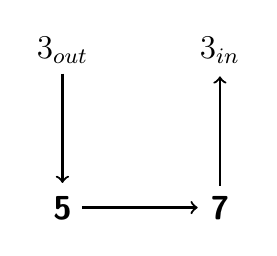
\begin{tikzpicture}[->,shorten >=1pt,auto,node distance=2cm,
            thick,main node/.style={font=\sffamily\large\bfseries}]

        % Define vertices
        \node[main node] (3) {$3_{in}$};
        \node[main node] (33) [left of=3] {$3_{out}$};
        \node[main node] (5) [below of=33] {5};
        \node[main node] (7) [below of=3] {7};
        

        % Draw edges
        \path[every node/.style={font=\sffamily\small}]
            (33) edge (5)
            (5) edge (7)
            (7) edge (3);

        \end{tikzpicture}
        \caption{SCC(C) split on 3}
        \label{fig:scc_c_split}
    \end{subfigure}
    \hfill
    \begin{subfigure}{0.45\textwidth}
        \centering
        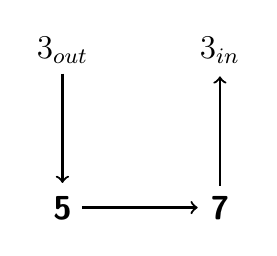
\begin{tikzpicture}[->,shorten >=1pt,auto,node distance=2cm,
            thick,main node/.style={font=\sffamily\large\bfseries}]

        % Define vertices
        \node[main node] (3) {$3_{in}$};
        \node[main node] (33) [left of=3] {$3_{out}$};
        \node[main node] (5) [below of=33] {5};
        \node[main node] (7) [below of=3] {7};
        

        % Draw edges
        \path[every node/.style={font=\sffamily\small}]
            (33) edge (5)
            (5) edge (7)
            (7) edge (3);

        \end{tikzpicture}
        \caption{condensed graph}
        \label{fig:condensed_scc_c_split}
    \end{subfigure}
    \caption{SCC(C) split on 3 and its condensed graph}
    \label{fig:scc_c_split_and_condensed_graph1}
\end{figure}

The figure \figureref{\ref{fig:scc_tree_graph1}} shows the SCC tree for the graph in \figureref{\ref{fig:graph1}}.
The SCC tree is constructed by the \textsc{MakeTree} algorithm, which recursively processes the condensed components of the split graph.
The child of each parent node in the SCC tree is a node present in the \textsc{STN} of the parent node.
\\$\textsc{SccTree(R)} = \textsc{STN}\text{'s of } \{R, 1, A, 2, C, 3, 5, 7, B, 4, 6, 8\}$


\begin{figure}[H]
    \centering
    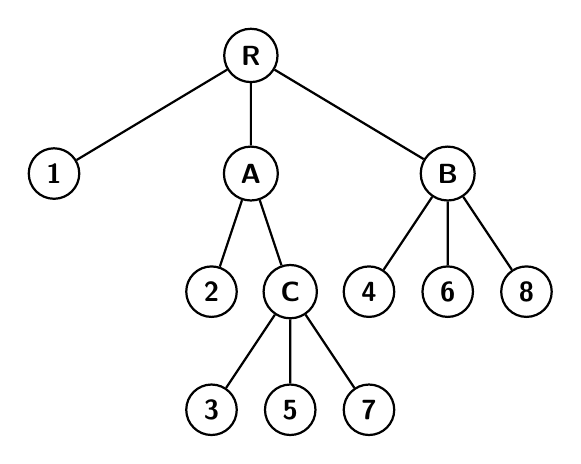
\begin{tikzpicture}[level distance=1.5cm,
                        level 1/.style={sibling distance=2.5cm},
                        level 2/.style={sibling distance=1cm},
                        thick,main node/.style={circle,draw,font=\sffamily\bfseries}]

      % Define vertices
      \node[main node] (R) {R}
        child {node[main node] (1) {1}}
        child {node[main node] (A) {A}
          child {node[main node] (2) {2}}
          child {node[main node] (C) {C}
            child {node[main node] (3) {3}}
            child {node[main node] (5) {5}}
            child {node[main node] (7) {7}}
          }
        }
        child {node[main node] (B) {B}
          child {node[main node] (4) {4}}
          child {node[main node] (6) {6}}
          child {node[main node] (8) {8}}
        };

    \end{tikzpicture}
    \caption{SCC Tree of Graph \ref{fig:graph1}}
    \label{fig:scc_tree_graph1}
\end{figure}

